\section{万有引力规律的建立}\label{sec:04.02}

在牛顿之前,已经有物体之间存在引力的观念,也有太阳的
引力决定行星运动的观念。但是怎样定量的描写引力?太阳引力
如何决定行星的运动?等等,都是不清楚的。

牛顿首先把他的动力学基本方程\eqref{eqn:03.02.01}~作为力的定义,来研
究导致开普勒三定律的力应是怎样的。

为了简便,可把行星轨道看作圆形。这样,根据面积定律,
% 127.jpg
行星应作匀速圆周运动,只有向心加速度
\begin{equation}\label{eqn:04.02.01}
	a = \frac { v ^ { 2 } } { r }  
\end{equation}
其中$ v $是行星的速率;$ r $是圆轨道的半径。根据开普勒第三定律
\lhbrak 式\eqref{eqn:04.01.01}\rhbrak 
\begin{equation*}
	T \propto r ^ { \frac { 3 } { 2 } }  
\end{equation*}

又注意到$ v = \frac { 2 \uppi r } { T }   $,故有
\begin{equation}\label{eqn:04.02.02}
	v \propto \frac { r } { r ^ \frac { 3 } {2}} = \frac { 1 } { r ^ {  \frac { 1 } { 2 } } }  
\end{equation}
将上式代入式\eqref{eqn:04.02.01},得
\begin{equation}\label{eqn:04.02.03}
	a \propto \frac { 1 } { r ^ { 2 } }  
\end{equation}
或
\begin{equation*}
	F = m a \propto \frac { m } { r ^ { 2 } }  
\end{equation*}
其中$ m $是行星的质量。取比例系数为$ \alpha $,则得
\begin{equation}\label{eqn:04.02.04}
	F = m \frac { \alpha } { r ^ { 2 } } 
\end{equation}
显然,$ \alpha $应取决于太阳的性质。由此,牛顿得到第一个重要结果:
如果太阳引力是行星运动的原因,则这种力应和$ r $的平方成反比。

在牛顿之前,也在人提出过引力应遵循平方反比律,但那并
不是基于力的明确定义而得到的,只是一种猜测,或者是与几何
类比而推出。在牛顿体系中,力具有定量的定义,再由运动学规
律及太阳是行星运动原因的模型,平方反比律就是必然的结论
了。

进一步,牛顿认为这种引力是万有的、普适的、统一的,即
所有物体之间都存在这种引力作用,称之为万有引力。这一步是
% 128.jpg
关键性的。我们一再强调,寻找各种不同运动的统一原因,是物
理学的追求,引力的万有性就是基于这种统一观的一种猜测。

如何来检验这一猜测呢?既然引力是普适的,那么,地球和
月亮之间也应当存在这类力,月亮之所以绕地球运动,应当是地
球施于月亮的吸引力,就象太阳有吸引行星的力那样,即地球对
月亮的吸引力也应当有式\eqref{eqn:04.02.04}~的形式,即
\begin{equation}\label{eqn:04.02.05}
	F _ { \text{地} \to \text{月}} = m _ {\text{月}} \frac { \alpha ' } { l ^ { 2 } }  
\end{equation}
显然,其中$ \alpha ' $应不同于式\eqref{eqn:04.02.04}~中的$ \alpha $,因为$ \alpha $标志太阳的性质,
而$ \alpha ' $应标志地球的性质。另外,在式\eqref{eqn:04.02.05}~中,$ m _ {\text{月}} $是月亮的质
量,$ l $是地球到月亮的距离。这时,月亮的加速度可表示为
\begin{equation}\label{eqn:04.02.06}
	a _ { \text{月} } = \frac { F _ { \text{地} \to \text{月}} } { m _ {\text{月}} } = \frac { \alpha ' } { l ^ { 2 } }  
\end{equation}
这里,是把动力学基本方程\eqref{eqn:03.02.01}~作为定律来使用。

另一方面,由式\eqref{eqn:04.02.05},地球对地面上落体的引力应是
\begin{equation}\label{eqn:04.02.07}
	F = m \frac { \alpha ' }  { R ^ { 2 } }  
\end{equation}
其中,$ m $是落体的质量,$ R $是地球半径。由此,落体的加速度$ g $
为
\begin{equation}\label{eqn:04.02.08}
	g = \frac { \alpha ' } { R ^ { 2 } }  
\end{equation}
从式\eqref{eqn:04.02.06}~及式\eqref{eqn:04.02.08},得
\begin{equation}\label{eqn:04.02.09}
	l = R \sqrt { { \frac { g } { a _ { \text{月} } }} }
\end{equation} 
又
\begin{equation*}
	a _ { \text{月} } = \frac { v ^ { 2 } } { l } \qquad  
v = \frac { 2 \uppi l } { T } 
\end{equation*}
其中,$ v $是月亮的速率;$ T $是月亮运动周期。将上式代入式\eqref{eqn:04.02.08}~
并整理,得到
% 129.jpg
\begin{equation}\label{eqn:04.02.10}
	l ^ { 3 } = \frac { 1 } { 4 \uppi ^ { 2 } } R ^ { 2 } g T ^ { 2 } 
\end{equation}
式\eqref{eqn:04.02.10}~就是从引力普适性得出的预言。在这个关系式中,所
有量都是可测量的,因此,可以用实验加以检验。其中有关量的
数值为
\begin{align*}
	R &\approx  6400 \text{公里} \\
	g &=  9.8 \text{米/秒} ^ 2 \\
	T &=  27 \text{天}8\text{小时} \\
	l &=  \num{3.84e5} \text{公里}
\end{align*}
这些测量结果能很好地满足式\eqref{eqn:04.02.10},这就验证了万有引力的
假设的正确性。

早在1665年,牛顿就得到了式\eqref{eqn:04.02.10},但用当时的测量数
据,牛顿发现它们并不满足式\eqref{eqn:04.02.10}。因而,牛顿并没有及时
发表他的成果。直到后来,天文学家重新测定了地球半径,发现
以前的观测值错了。牛顿用新的数据再进行计算,所得结果完全
符合式\eqref{eqn:04.02.10} 。这可能是牛顿推迟发表他的万有引力理论的一
个原因。

牛顿的上述论证说明,地上物体的运动规律与月亮运动的规
律实质上是一样的。这个结果的意义很重大,它打破了亚里士多
\begin{wrapfigure}[9]{r}{10.5em}
	\centering
	\vspace{-1em}
	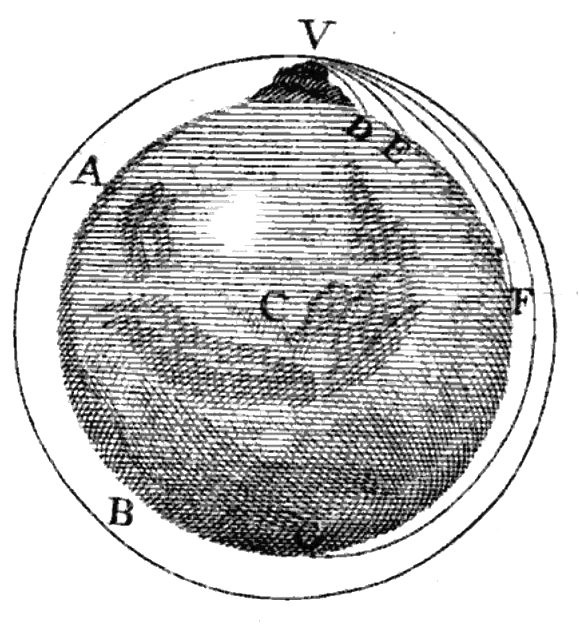
\includegraphics[width=10em]{figure/fig04.03}
	\caption{天体运动和地面运动无原则差别}
	\label{fig:04.03}
\end{wrapfigure}	
德关于天上运动和地面运动是本质不
同的两类运动的基本观念。按照牛顿
的理论,天体运动与地面运动之间并
无根本的差别,也没有不可渡过的界
限。牛顿曾描述过在高山顶上用大炮
发射炮弹的运动情形,见图\ref{fig:04.03}。我们
知道,炮弹作抛体运动。按牛顿理论,
只要炮弹的初速度足够大,炮弹就能
绕地球运动,而不再落回地面,成为
% 130.jpg
地球的卫星。因此落体或抛体运动与地球卫星的运动之间的差
别,只不过是初速度不同。今天看来,这些结果已没有什么希奇,
因为已经成功地发射了很多人造地球卫星。但在三百多年前,就
认为原则上我们可制造天体那样的运动,是一个非常大胆的想
法。

上面的讨论我们只利用了开普勒的第二、第三定律,还应当
证明万有引力定律式\eqref{eqn:04.02.04}~或式\eqref{eqn:04.02.05}~也符合开普勒的轨道定
律。牛顿在1677年完成了这个证明,使万有引力理论形成了完整
的体系。关于轨道定律的证明,已超出本课程的范围,故不在这
里论述这个证明过程了。

牛顿在他的小传中,总结过自己这一段的工作,他说:“在
1665年开始……我从开普勒关于行星的周期是和行星到轨道中心
的距离的3/2次方成比例的定律,推出了使行星保持在它们的轨道
上的力必定和它们与绕行中心之间的距离平方成反比;尔后,把使
月球保持在它轨道上所需要的力和地球表面上的重力作了比较,
并发现它们近似相等。所有这些发现都是在1665和1666的鼠疫年
代里作出来的……最后在1676和1677年之间的冬季,我发现了一
个命题,那就是——一个行星必然要作一个椭圆形的运动,力心
在椭圆的一个焦点上,同时,它所扫过的面积(从力心算起)的大
小和所用的时间成正比。”从这个总结中,我们可以看到,“从
运动现象研究力,再从力去说明其他现象”的完整过程。这种物
理的研究方法一直沿用到今天。
